\documentclass[11pt]{article}
\usepackage[margin=0.75in]{geometry}
\usepackage{graphicx}
\usepackage{hyperref}
\usepackage{enumitem}
\usepackage{listings}

\lstdefinestyle{mystyle}{
    basicstyle=\ttfamily\footnotesize,
    breakatwhitespace=false,         
    breaklines=true,                 
    keepspaces=true,                 
    showspaces=false,                
    showstringspaces=false,
    showtabs=false,                  
    tabsize=2
}

\lstset{style=mystyle}

\begin{document}

\title{Ling 282/482 hw2}
\date{\vspace{-0.2in}Due 11PM on October 6, 2025}
\maketitle


In this assignment, you will answer some written questions about Word2Vec and then analyze the provided PyTorch implementation. In particular, we employ  the method called \emph{Skip-Gram with Negative Sampling (SGNS)}. By doing so you will:
\begin{itemize}
  \item Count parameters
  \item Take derivatives of a loss
  \item See how mathematics and Python code correspond
  \item Train your own set of word vectors and briefly analyze them
\end{itemize}

\section*{Submission Instructions}
\noindent Please answer the following questions and submit your answers \textbf{as a PDF on Blackboard}. Note that for Part 2, Q2, you have the option of uploading your edited code files instead of including the answers directly in your writeup. Your final submission will be the one that is graded unless you specify otherwise.


\section{Understanding Word2Vec [30 pts]}

\noindent {\bf Q1: Parameters [2 pts]}  How many parameters are there in the SGNS model?  Write your answer in terms of $V$ (the vocabulary) and $d_e$, the embedding dimension.  (Hint: one parameter is \emph{a single real number}.)

\vspace{2em}
\noindent {\bf Q2: Sigmoid [8 pts]}  Sigmoid is the logistic curve $\sigma(x) = \frac{1}{1+e^{-x}}$.
\begin{itemize}
  \item What is the range of $\sigma(x)$? [2 pts]
  \item How is it used in the SGNS model? [2 pts]
  \item Show that $\frac{d}{dx}\sigma(x) = \sigma(x)(1-\sigma(x))$ [4pts]
\end{itemize}

\vspace{2em}
\noindent {\bf Q3: Loss function's gradients [20 pts]}  In the slides for lecture 3, we saw that the total loss for one positive example and $k$ negative examples is given by:
$$ L_{CE} = -\log P(1 | w, c_+) - \sum_{i=1}^k \log P(0 | w, c_{-i})$$
In what follows, where $x$ is a vector and $f$ a function of $x$ and possibly more variables, we will define $\nabla_x f := \langle \frac{\partial f}{\partial x_1} , \frac{\partial f}{\partial x_2}, \dots , \frac{\partial f}{\partial x_n} \rangle$.
\begin{itemize}
  \item Rewrite this loss in terms of the parameter matrices $E$ and $C$ (i.e. replace the $P(\cdot)$s with the definition of the model). [2 pts]

        Use $w$ as the integer index of the target word, $c_+$ as the integer index of the positive context word, and $c_{-i}$ as the integer index of the $i$th negative sampled context word.
  \item Using the chain rule, compute $\frac{d}{dx} -\log\sigma(x)$.  (Hint: first, show that $\sigma(x) = \frac{e^x}{e^x+1}$.  Note: $\log$ here is the natural logarithm, i.e. logarithm with base $e$.) [4 pts]
  \item Show that $\nabla_x x \cdot y = y$ (where $x \cdot y$ is the dot product of two vectors). [2 pts]
  \item Compute (and show your work) $\nabla_{C_{c_+}} L_{CE}$. [4 pts]
  \item Compute (and show your work) $\nabla_{C_{c_{-i}}} L_{CE}$. [4 pts]
  \item Compute (and show your work) $\nabla_{E_w} L_{CE}$. [4 pts]
\end{itemize}

\section{Word2Vec Implementation [46 pts]}
\noindent {\bf Q1: Get access to the code [6 pts]} 
\begin{enumerate}[label=\alph*.]
  \item Sign up for a \href{https://github.com}{Github account} if you don't yet have one. Then \textbf{send your username to your instructor}, either by email or Blackboard messages. You will be added to the Github repository for this homework, containing the word2vec code which you will answer questions about.
  \item \textbf{Create a fork} of the repository. This can be done from the home page of the repository under the button that says ``Fork'' (see screenshot below). This will create your own working copy of the code that you can clone your local machine or BlueHive and edit.
  \item \textbf{Clone your fork to BlueHive}. On the home page of your fork, there will be a green button that says ``Code''. Under the ``Clone'' section, there will be an option to copy an HTTPS address to your clipboard. On BlueHive, navigate to your \textbf{personal scratch folder}. Then run the command \texttt{git clone <address>} where \texttt{<address>} is replaced by the url you just copied. You will be prompted to enter your Github username and password before the repository is cloned.
\end{enumerate}

\begin{figure}[h!]
  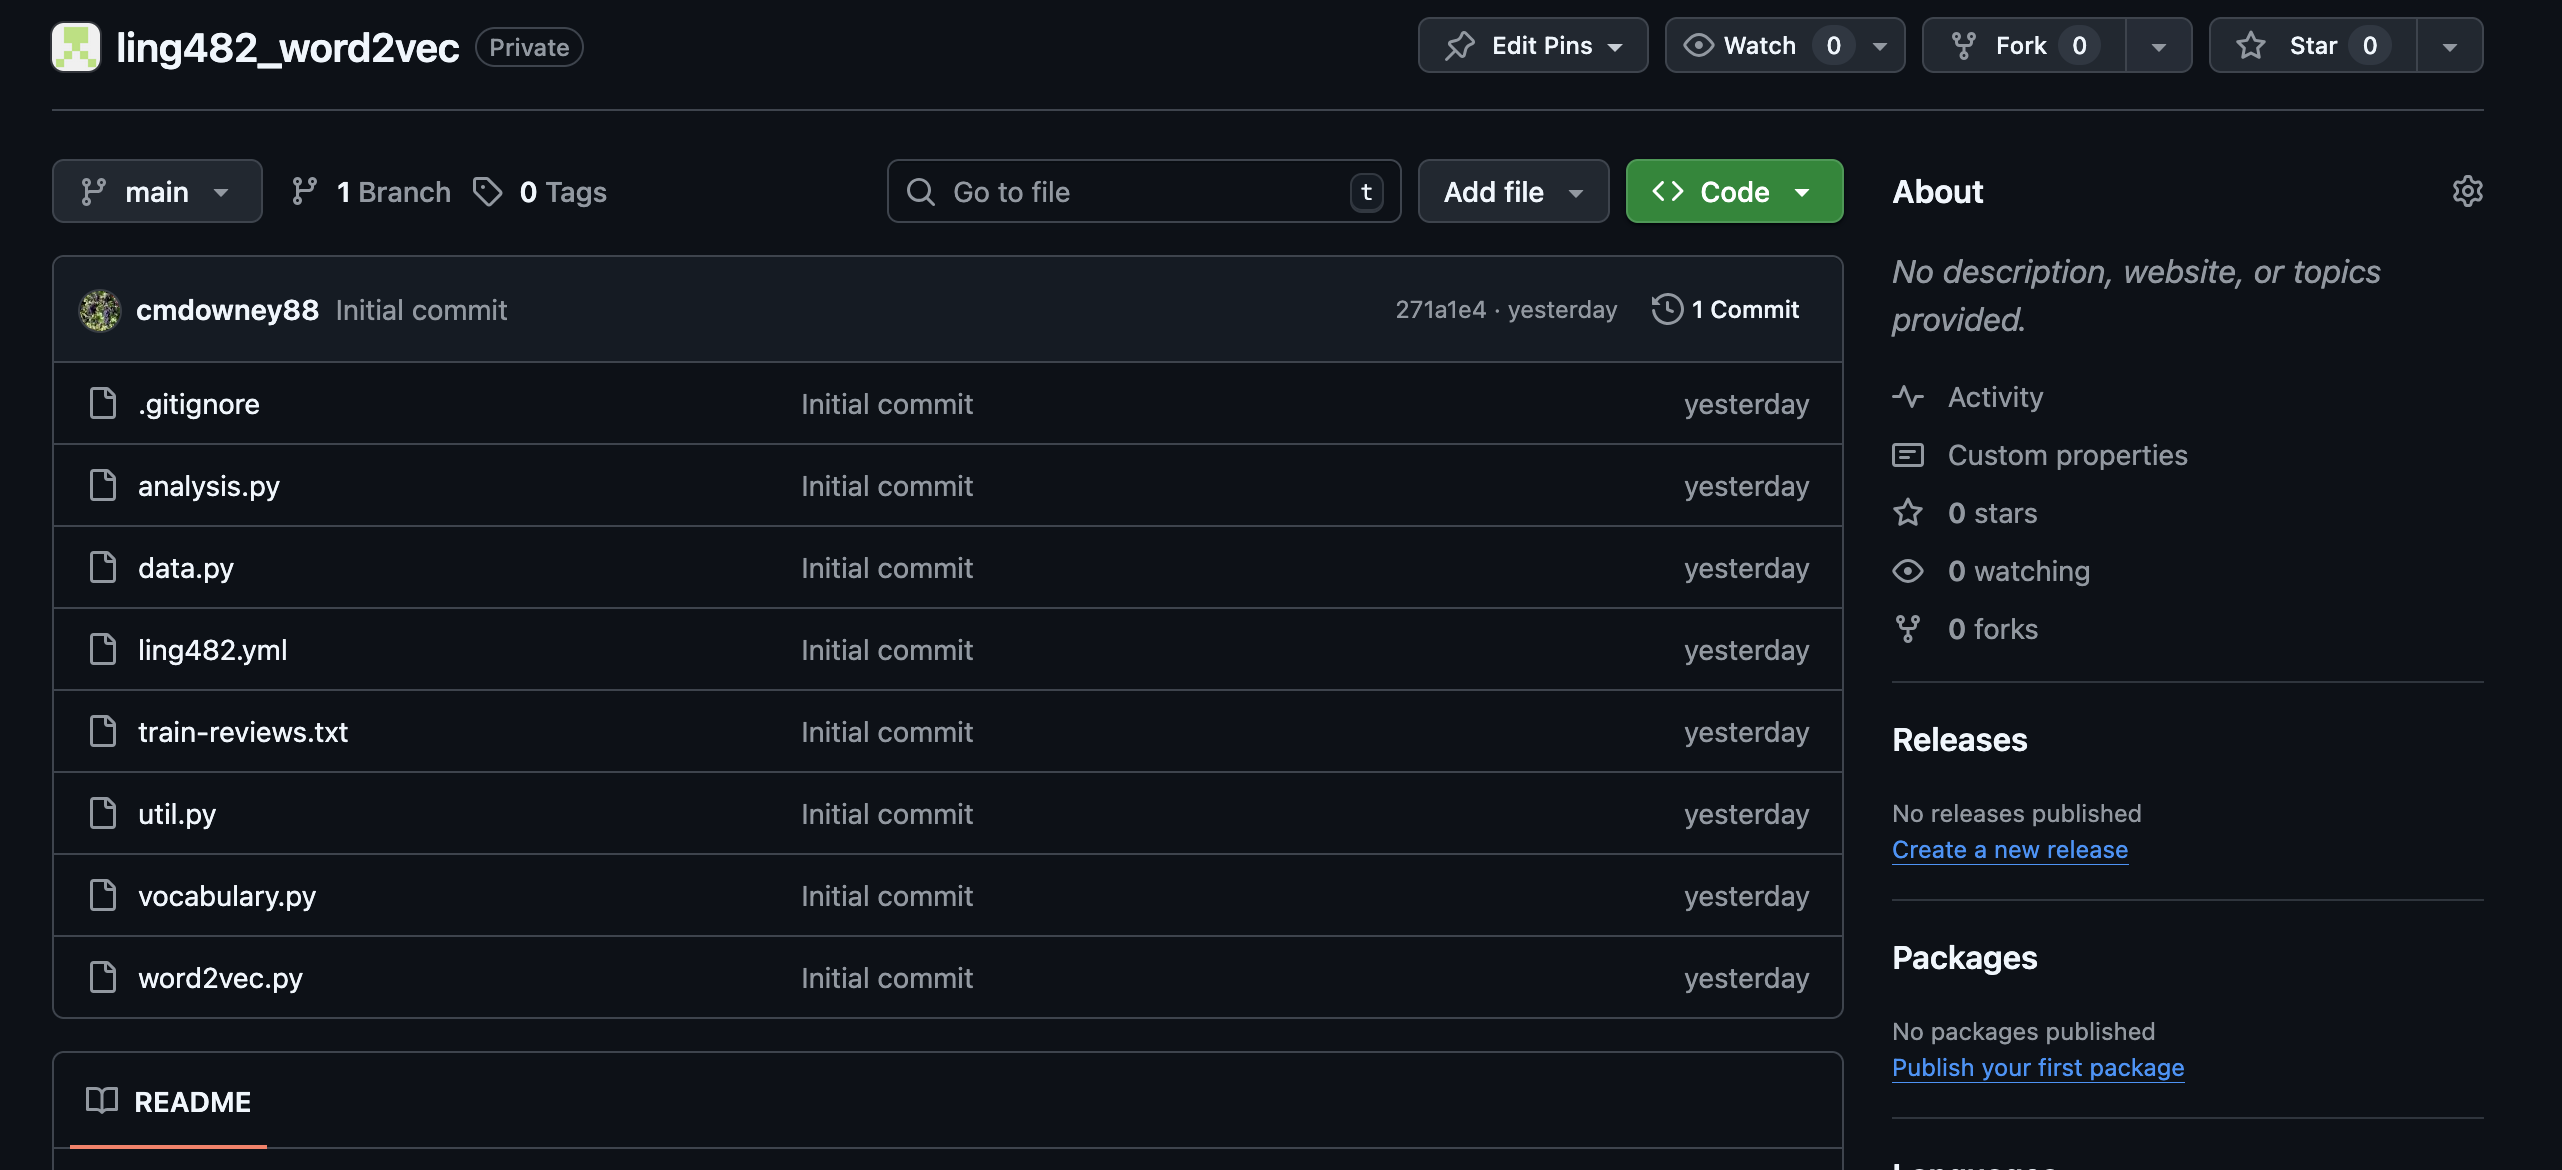
\includegraphics[width=0.9\textwidth]{repo_buttons.png}
  \centering
\end{figure}

\newpage
\noindent {\bf Q2: Write Docstrings [16 pts]} In quality Python code, functions/methods and classes should always be documented with \textit{Docstrings}. Docstrings are long comments that come immediately after the function/class definition and describe 1) the overall functionality 2) the \textit{arguments} that the function takes in (including their types), and 3) what the function \textit{returns}, including the return type. Some examples of completed docstrings can be found in \texttt{data.py}, e.g. for the function \texttt{generate\_training\_data}. For this question, you will \textbf{fill in the missing docstrings} for the following functions and methods:

\begin{itemize}
  \item \texttt{negative\_samples} (\texttt{data.py}) [4 pts]
  \item \texttt{negatives\_from\_positives} (\texttt{data.py}) [4 pts]
  \item \texttt{get\_positive\_samples} (\texttt{data.py}) [4 pts]
  \item \texttt{SGNS.forward} (\texttt{word2vec.py}) [4 pts]
\end{itemize}

\textbf{HINTS:} The main script for running the word2vec algorithm is in \texttt{word2vec.py}. This script uses the functions defined in \texttt{data.py} to pre-process the data for input ot the model. In writing your docstrings, it will help you to understand \textbf{how these functions are being used} in \texttt{word2vec.py}. These data functions are also described in more general terms in the word2vec course slides.

You can submit your work \textbf{either} by writing your docstrings in the area below in the LaTeX document (just the docstrings, not the actual code), or by writing the docstrings directly in your copy of the code, and uploading the modified versions of \texttt{data.py} and \texttt{word2vec.py} to Blackboard along with your PDF writeup. Indicate which option you are choosing in your writeup.

\begin{lstlisting}
def get_positive_samples(
    text: list[str], window_size: int, tokens: list[str]
) -> list[tuple[str, str]]:
    """TODO: your docstring summary here

    Args:
        TODO: document the arguments

    Returns:
        TODO: document what the function returns
    """
\end{lstlisting}

\vspace{2em}
\noindent {\bf Q3: Understanding the model implementation [16 pts]}
\begin{enumerate}[label=\alph*.]
  \item In \texttt{SGNS.forward}, what are lines 32-34 doing? (These are the lines that call \texttt{torch.mul} and \texttt{torch.sum}). In other words, how do these lines relate to the definition of the SGNS model described in the slides? [4 pts]
  \item Where are the gradients that you calculated in Part 1 of this homework actually calculated within the code? Hint: it is a single line of \texttt{word2vec.py}. Describe what this line is doing. [2 pts]
  \item What does the command \texttt{optimizer.step()} do? (\texttt{word2vec.py}, line 94) [2 pts]
  \item In lines 83-84 (\texttt{word2vec.py}), we define the variable \texttt{batch\_y}. What is the purpose of this variable? What does it correspond to in the slides? [4 pts]
  \item Look up the PyTorch documentation for \texttt{BCEWithLogitsLoss}. How does it relate to the loss function we described in the slides, and why are we using it here? [4 pts]
\end{enumerate}

\newpage
\noindent {\bf Q4: Train word vectors [8 pts]} Now you will run the training script you've been inspecting to produce word vectors. You should run this code \textbf{on BlueHive}, within an interactive session. Reminder: to start an interactive session, you need to run the command \texttt{interactive -c 20 --mem=64g}. Once in the interactive session, make sure to activate the course Python environment. Run the main training loop by running the command \texttt{python word2vec.py}. The default hyper-parameters for the training loop can be found at the very bottom of the training script. The training will take \textbf{about 15 minutes}. \textbf{Notice:} this script might not output anything for a few minutes after you first run it. It should be quicker if you run it subsequent times.

After that, run \texttt{python analysis.py --save\_vectors vectors.tsv --save\_plot vectors.png}.  This will take your saved vectors and produce a plot with the vectors (after using PCA to reduce dimensionality to 2) of a select choice of words.  In your writeup, please include: 
\begin{itemize}
  \item The total run-time of your training loop.  This will be printed by the main script.
  \item The generated plot.
  \item Describe in 2-3 sentences any trends that you see in these embeddings.
\end{itemize}

\noindent \textbf{Hint:} A file can be copied from BlueHive to your local computer by runninig the following command in a \textbf{local terminal session.} You will have to enter your password and Duo 2FA. Note the dot \texttt{.} at the end of the command. The dot is shorthand for ``here'' (whichever folder you're in on your local computer).

\noindent \texttt{scp username@bluehive.circ.rochester.edu:/scratch/username/foldername/filename .}

\section{Understanding Computation Graphs [24 pts]}

\noindent {\bf Q1: Worked example}  Consider the function $f(x) = x^2 \times cx$.
\begin{itemize}
  \item Draw a computaton graph for this expression. [4 pts]
  \item How many nodes are there (including input and output)? [2 pts]
  \item For $x = 2$ and $c=3$: [12 pts]
    \begin{itemize}
      \item Compute the value of each node in a forward pass.
      \item Compute $\frac{df}{dn}$ for each node $n$, using backpropagation.
    \end{itemize}
  \item Consider the node corresponding to $x^2$ in the graph.  For each of the following, write a symbolic expression and the numerical value (at $x=2$, $c=3$) for: [6 pts]
    \begin{itemize}
      \item The upstream derivative.
      \item The local derivative.
      \item The downstream derivative(s).
    \end{itemize}
\end{itemize}

%%%%%%%%%%%%%%%%%%%%%%%%%%%%%%%

\end{document}
